\documentclass[conference]{IEEEtran}
\IEEEoverridecommandlockouts

\usepackage{url}
\usepackage{cite}
\usepackage{tikz}
\usetikzlibrary{positioning, fit, arrows.meta, calc}
\usepackage{amsmath,amssymb,amsfonts}
\let\proof\undefined
\let\endproof\undefined
\usepackage{amsthm}
\usepackage{algorithm}
\usepackage{algpseudocode}
\usepackage{graphicx}
\usepackage{textcomp}
\usepackage{xcolor}
\usepackage{booktabs}

\let\oldtextsc\textsc
\renewcommand{\textsc}[1]{\textup{\oldtextsc{#1}}}
\setlength{\emergencystretch}{2em}

\newtheorem{proposition}{Proposition}
\newtheorem{theorem}{Theorem}
\newtheorem{lemma}{Lemma}
\newtheorem{corollary}{Corollary}
\newtheorem{definition}{Definition}

\def\BibTeX{{\rm B\kern-.05em{\sc i\kern-.025em b}\kern-.08em
		T\kern-.1667em\lower.7ex\hbox{E}\kern-.125emX}}

\begin{document}
	
	\title{Cuckoo Hashing with Bounded Displacement for Exact-Match Flow Tables}
	
	\author{\IEEEauthorblockN{Soumyajit Kolay}
		\IEEEauthorblockA{\textit{School of Computer Engineering} \\
			\textit{KIIT Deemed University}\\
			Bhubaneswar, India \\
			2650026@kiit.ac.in}
	}
	
	\maketitle
	
	% ======================================================================
	% ABSTRACT -- human-written. Insert here.
	% ======================================================================
	
	\begin{abstract}
		This paper deals in discussing a variant of $d$-ary Cuckoo Hashing Tables that considers bounded displacement to ensure a higher value for recommended load, on which it does with lesser number of full rehashes as compared to previous algorithms. This paper is still in progress and serves as a \LaTeX learning playground for the author.
	\end{abstract}
	
	\begin{IEEEkeywords}
		Software-Defined Networking, Flow Tables, Cuckoo Hashing, Bounded Displacement, Stash Mechanisms, Deterministic Latency, Line-Rate Packet Processing
	\end{IEEEkeywords}
	
	% ======================================================================
	% I. INTRODUCTION -- human-written. Insert here.
	% Outline + citation list + terms-to-define already agreed on separately;
	% not reproduced in this file per your instruction.
	% ======================================================================
	
	\section{Introduction}
	Para 1 — "Exact-Match Flow Tables."
	line-rate dictionary requirement; fixed per-packet time budget
	
	\subsection{Literature Review}
	Para 2 — "Classical Cuckoo Hashing."
	Pagh-Rodler; 2-way displacement; O(1) worst-case lookup
	
	Para 3 — "The Full-Rehash Catastrophe."
	$MaxLoop = \Theta(log n)$; O(n) full rehash; why that's unacceptable at line rate
	
	Para 4 — "Stash-Based Mitigation." (chronological)
	Kirsch/Kutzelnigg/Aumüller/Fountoulakis-Panagiotou — reduces rehash odds,
	but all still assume unbounded search before stash
	
	Para 5 — "Networking-Specific Variants." (chronological)
	Pontarelli x2/Le Scouarnec/Kuszmaul/Noble/Minaud-Papamanthou/TECache —
	throughput/energy-focused, no worst-case insertion bound
	
	[one-line forward pointer: Sec. II quantifies baseline rehash frequency first]
	
	\subsection{Implementation-Driven Corrections}
	Building a reference implementation surfaced one correctness issue not
	apparent from the pseudocode alone. The initial \textsc{RehashStash}
	design redrew a fresh global hash-function tuple on every stash
	overflow and reinserted only the stashed key(s). This silently orphaned
	every key already resident in the main tables: their physical slot had
	been computed under the \emph{old} hash functions, so a lookup issued
	under the new ones would almost never find them. The anomaly first
	appeared as an implausible positive-lookup probe-count distribution
	rather than as an outright failure, and was only isolated with a
	standalone occupancy diagnostic that showed the physical key
	distribution contradicted the reported lookup behavior. The corrected
	design keeps the global hash functions fixed for the table's lifetime
	and instead retries the stashed key's bounded-kick placement with
	fresh \emph{randomized eviction choices} only -- simpler than the
	original design, and it removes the hazard entirely while preserving
	the $O(s)$ incremental-rehash cost. A small recursion-depth guard was
	added defensively against pathological repeated-retry cases, though it
	was never observed to trigger.
	
	A second, lower-level lesson concerned evaluation honesty rather than
	correctness: a single benchmark point near Pagh--Rodler's own
	conservative recommended load ($\alpha\!\approx\!1/3$) shows
	essentially zero full rehashes for the classical baseline, which would
	understate the exact failure mode this paper is motivated by. Only
	sweeping load factor toward the $d$=2 structural ceiling
	($\alpha\!\approx\!0.495$) surfaces the real tail blow-up, indicating
	that near-ceiling operating points must be tested explicitly rather
	than only "typical" ones.
	
	\subsection{Contributions}
	Para 7 — "Contributions."
	bulleted, each tagged to its section.
	
	\section{Modeling Rehash Frequency in Classical Cuckoo Hashing}
	\label{sec:modeling}
	
	Before presenting the proposed design, this section quantifies the
	failure mode it targets. In classical $2$-way cuckoo hashing, an
	insertion's eviction loop is bounded by
	$\mathtt{MaxLoop} = \lceil 3\log_{1+\varepsilon} r \rceil$, where
	$r=(1+\varepsilon)n$ is the table capacity~\cite{pagh2004cuckoo}. Pagh and
	Rodler show the probability that a single insertion exhausts
	$\mathtt{MaxLoop}$ -- and therefore triggers a full-table rehash -- is
	bounded by
	\begin{equation}
		\Pr[\text{rehash triggered}] \le 2(1+\varepsilon)^{-\frac{2\cdot\mathtt{MaxLoop}-1}{3}+1} + O(n^{-2}),
		\label{eq:baseline-rehash-prob}
	\end{equation}
	the same path-counting bound used later in
	Section~\ref{sec:theory}B, evaluated here at $t=\mathtt{MaxLoop}$ instead
	of a fixed constant. Because $\mathtt{MaxLoop}$ grows with $n$, this
	probability is small \emph{in the asymptotic limit} -- but $\varepsilon$
	is fixed by the table's slack at construction time, and for a given
	finite $n$ the realized rehash frequency depends heavily on how close
	the load factor $\alpha=n/r$ sits to the $d$-ary structural ceiling
	(e.g.\ $\approx 50\%$ for $d=2$~\cite{pagh2004cuckoo}). Eq.~\ref{eq:baseline-rehash-prob}
	predicts that rehash frequency should rise sharply as $\alpha$
	approaches that ceiling, independent of $n$'s asymptotic comfort.
	
	This prediction is checked directly against a reference implementation
	in Section~\ref{sec:eval}: TBD (\emph{technique}: measured directly from
	the classical-cuckoo baseline in \texttt{bench.cpp} at two operating
	points -- Pagh and Rodler's own recommended $\alpha\!\approx\!1/3$, and
	a point near the $d{=}2$ ceiling, $\alpha\!\approx\!0.49$--$0.495$;
	see Section~\ref{sec:eval}B). As with the modeling-before-design pattern
	this section follows, Eq.~\ref{eq:baseline-rehash-prob} is not claimed
	to predict exact rehash counts under correlated or adversarial
	insertion orderings -- it motivates \emph{why} full-table rehashing is
	the right failure mode to target, and gives a closed-form baseline the
	proposed scheme's own bounds (Section~\ref{sec:theory}) are compared
	against. The remainder of the paper addresses this failure mode
	structurally rather than by tuning $\varepsilon$ or $\mathtt{MaxLoop}$
	alone (see the Discussion, Section~\ref{sec:discussion}, for why tuning
	$\mathtt{MaxLoop}$ down is not by itself a solution).
	
	\section{System Architecture \& Proposed Algorithm}
	\label{sec:algorithm}
	
	\subsection{Design Goals}
	Bounding the eviction chain and introducing a stash is a structural
	departure from classical cuckoo hashing, and that departure introduces
	four concerns that did not exist in the unbounded scheme. The
	remainder of this paper is organized around resolving each:
	\begin{enumerate}
		\item[\textbf{G1}] \textbf{Bounded worst-case latency.} Every
		insertion must complete in time independent of $n$
		(Section~\ref{sec:theory}A).
		\item[\textbf{G2}] \textbf{Rehash correctness.} Giving a stashed key
		a fresh placement attempt must never silently break lookups for
		keys already resident in the main tables
		(Section~\ref{sec:algorithm}C, Section~\ref{sec:discussion}).
		\item[\textbf{G3}] \textbf{Bounded stash pressure.} $\mathtt{MaxKicks}$
		and stash capacity $s$ must be sized jointly against a quantified
		stash-routing probability, not chosen arbitrarily
		(Section~\ref{sec:theory}B--C, Section~\ref{sec:eval}D).
		\item[\textbf{G4}] \textbf{Load-factor coupling.} $\mathtt{MaxKicks}$,
		$s$, and the $d$-ary load threshold are not independent knobs;
		operating near the hypergraph's structural ceiling changes the
		whole routing-probability profile (Section~\ref{sec:theory}D).
	\end{enumerate}
	
	\subsection{Formal Mathematical Definitions \& System Model}
	Let $U = \{0, 1\}^w$ be the universe of $w$-bit flow identifiers (e.g.,
	standard IPv4 5-tuples)~\cite{pagh2004cuckoo}. An exact-match flow table
	consists of $d \ge 2$ independent sub-tables $T_1, \dots, T_d$, each
	containing $m$ slots~\cite{pagh2004cuckoo}. The total capacity of the
	main table is $r = dm$ slots. The table maintains $n = |S|$ active
	microflows from a set $S \subset U$. The overall load factor is
	\begin{equation}
		\alpha = \frac{n}{r} = \frac{n}{dm}.
	\end{equation}
	The dictionary uses $d$ uniform, independent hash functions drawn from
	a universal hash family $\mathcal{H}$:
	\begin{equation}
		h_i : U \to \{0, 1, \dots, m-1\}, \quad \forall i \in \{1, \dots, d\}.
	\end{equation}
	Every stored flow key $x \in S$ resides either in one of its $d$
	candidate sub-table locations $T_i[h_i(x)]$ or in an auxiliary stash
	$\text{Stash}$ of capacity $s \ll n$~\cite{kirsch2009stash}. Empty table
	slots are denoted $\bot$. Hash functions $h_1,\dots,h_d$ are fixed for
	the table's lifetime once any key has been placed under them (see
	Algorithm~\ref{alg:rehashstash} and G2 above).
	
	\subsection{Algorithmic Specifications}
	
	\begin{algorithm}[t]
		\caption{\textsc{Lookup}$(x)$}
		\label{alg:lookup}
		\begin{algorithmic}[1]
			\For{$i \gets 1$ to $d$}
			\If{$T_i[h_i(x)] = x$}
			\State \Return \textsc{Found}
			\EndIf
			\EndFor
			\For{each entry $e$ in \textsc{Stash}}
			\If{$e = x$}
			\State \Return \textsc{Found}
			\EndIf
			\EndFor
			\State \Return \textsc{NotFound}
		\end{algorithmic}
	\end{algorithm}
	
	\begin{algorithm}[t]
		\caption{\textsc{Insert}$(x)$}
		\label{alg:insert}
		\begin{algorithmic}[1]
			\If{\textsc{Lookup}$(x) = \textsc{Found}$}
			\State \Return \textsc{AlreadyPresent}
			\EndIf
			\If{$(n+1)/(dm) > \textsc{LoadThreshold}(d)$} \Comment{\cite{fountoulakis2012sharp}}
			\State \textsc{Resize}()
			\EndIf
			\State $cur \gets x$
			\For{$round \gets 1$ to $\mathtt{MaxKicks}$} \Comment{constant, independent of $n$}
			\For{$i \gets 1$ to $d$}
			\If{$T_i[h_i(cur)] = \bot$}
			\State $T_i[h_i(cur)] \gets cur$; \quad $n \gets n+1$
			\State \Return \textsc{Success}
			\EndIf
			\EndFor
			\State $i \gets \textsc{ChooseCandidateIndex}(cur)$ \Comment{uniform random}
			\State $evicted \gets T_i[h_i(cur)]$; \quad $T_i[h_i(cur)] \gets cur$
			\State $cur \gets evicted$
			\EndFor
			\If{\textsc{Stash} has a free slot}
			\State place $cur$ in \textsc{Stash}; \quad $n \gets n+1$
			\State \Return \textsc{Success} \Comment{via stash}
			\EndIf
			\State \textsc{RehashStash}() \Comment{incremental --- Alg.~\ref{alg:rehashstash}}
			\State \Return \textsc{Insert}$(x)$ \Comment{retry; depth-guarded, see Alg.~\ref{alg:rehashstash}}
		\end{algorithmic}
	\end{algorithm}
	
	\begin{algorithm}[t]
		\caption{\textsc{RehashStash}()}
		\label{alg:rehashstash}
		\begin{algorithmic}[1]
			\State $S \gets$ contents of \textsc{Stash}; empty \textsc{Stash}
			\For{each key $y \in S$}
			\State reinsert $y$ via \textsc{Insert}, \emph{same} $h_1,\dots,h_d$
			\Comment{fresh randomized eviction path only -- see G2, Sec.~\ref{sec:discussion}}
			\EndFor
		\end{algorithmic}
	\end{algorithm}
	
	\begin{algorithm}[t]
		\caption{\textsc{Delete}$(x)$}
		\label{alg:delete}
		\begin{algorithmic}[1]
			\For{$i \gets 1$ to $d$}
			\If{$T_i[h_i(x)] = x$}
			\State $T_i[h_i(x)] \gets \bot$; \quad $n \gets n-1$; \quad \Return \textsc{Success}
			\EndIf
			\EndFor
			\If{$x \in$ \textsc{Stash}}
			\State remove $x$ from \textsc{Stash}; \quad $n \gets n-1$; \quad \Return \textsc{Success}
			\EndIf
			\State \Return \textsc{NotFound}
		\end{algorithmic}
	\end{algorithm}
	
	Two design points distinguish Algorithm~\ref{alg:insert} from the
	classical procedure of Pagh and Rodler~\cite{pagh2004cuckoo}. First, the
	outer loop is bounded by $\mathtt{MaxKicks}$, a constant fixed
	independently of $n$, in place of
	$\mathtt{MaxLoop} = \lceil 3\log_{1+\varepsilon} r \rceil$, which grows
	logarithmically with table size. Second, reaching this bound routes the
	displaced key to the stash rather than discarding all hash functions
	and reinserting every key in the table. \textsc{RehashStash}
	(Algorithm~\ref{alg:rehashstash}) reinserts only the keys currently
	held in the stash, \emph{without} redrawing $h_1,\dots,h_d$: a prior
	version of this routine drew a fresh hash-function tuple on every
	overflow, which silently broke lookups for every key already resident
	in the main tables, since their physical slot had been computed under
	the old functions (see Section~\ref{sec:discussion} for the full
	account). The corrected version relies only on
	\textsc{ChooseCandidateIndex}'s randomization for a fresh placement
	attempt. A small recursion-depth guard (not shown) falls back to a
	full rehash after a fixed number of failed retries; TBD whether this
	fallback is ever exercised in practice at the load factors tested in
	Section~\ref{sec:eval} (\emph{technique}: instrument the guard's trip
	counter in \texttt{bench.cpp} and report it alongside Table~\ref{tab:comparative_performance}).
	
	\section{Theoretical Analysis}
	\label{sec:theory}
	
	This section establishes: a deterministic worst-case $O(1)$ bound on
	per-insertion latency (Theorem~\ref{thm:worst_case_latency}), a
	closed-form upper bound on per-insertion stash-routing probability
	(Lemma~\ref{lem:stash_routing_prob}), a stash-overflow probability
	bound via multiplicative Chernoff inequalities
	(Theorem~\ref{thm:stash_overflow_bound}), and the amortized cost of
	incremental rehashing (Lemma~\ref{lem:rehash_cost}).
	
	\subsection{Worst-Case Insertion Latency}
	
	\begin{proposition}[Classical Worst-Case Insertion Latency]
		In the classical construction of~\cite{pagh2004cuckoo}, a single call
		to \textsc{Insert} performs $\Theta(\log n)$ work in the worst case
		before either succeeding or triggering a full-table rehash.
	\end{proposition}
	\begin{proof}
		$\mathtt{MaxLoop} = \lceil 3\log_{1+\varepsilon} r \rceil$ is chosen
		so the probability of exhausting it is $O(n^{-2})$ per insertion
		(Section~2.3 of~\cite{pagh2004cuckoo}). Because $\mathtt{MaxLoop}$
		grows logarithmically with $n$, the worst-case work per insertion
		scales as $\Theta(\log n)$.
	\end{proof}
	
	\begin{theorem}[Worst-Case $O(1)$ Insertion Latency]
		\label{thm:worst_case_latency}
		Every call to \textsc{Insert} (Algorithm~\ref{alg:insert}) performs
		at most $d\cdot\mathtt{MaxKicks}+O(1)$ hash evaluations, cell probes,
		and displacements before returning \textsc{Success} or invoking
		\textsc{RehashStash}. Since $d$, $s$, and $\mathtt{MaxKicks}$ are
		fixed constants, a single \textsc{Insert} call runs in deterministic
		$O(1)$ worst-case time, exclusive of the amortized
		\textsc{RehashStash} cost (Lemma~\ref{lem:rehash_cost}).
	\end{theorem}
	\begin{proof}
		\textsc{Lookup} costs $d+s=O(1)$ probes. The load check is $O(1)$.
		The eviction loop runs at most $\mathtt{MaxKicks}$ rounds, each
		costing $O(d)$ probes plus $O(1)$ swap work, for
		$O(d\cdot\mathtt{MaxKicks})$ total. Stash placement costs $O(s)=O(1)$.
		Summing: $T_{\text{insert}}(n) \le O(d\cdot\mathtt{MaxKicks}+s)=O(1)$,
		independent of $n$. The recursive retry (Algorithm~\ref{alg:insert},
		last line) executes only on stash overflow, bounded separately in
		Theorem~\ref{thm:stash_overflow_bound}.
	\end{proof}
	
	\subsection{Stash-Routing Probability and Stash Sizing}
	
	\begin{lemma}[Per-Insertion Stash-Routing Probability]
		\label{lem:stash_routing_prob}
		Let $h_1,\dots,h_d$ be drawn from an $(O(1),O(\mathtt{MaxKicks}))$-universal
		family, with $r=dm=(1+\varepsilon)n$ (base case $d=2$). The
		probability that a single insertion performs $\mathtt{MaxKicks}$
		displacements without locating an open slot satisfies
		\begin{equation}
			p(\mathtt{MaxKicks},\varepsilon) \le 2(1+\varepsilon)^{-\frac{2\cdot\mathtt{MaxKicks}-1}{3}+1} + O(n^{-2}).
		\end{equation}
	\end{lemma}
	\begin{proof}
		Adapting the three-case decomposition of~\cite{pagh2004cuckoo}
		(hash-family non-independence, closed-cycle traversal, long
		nestless-path formation) at a fixed threshold $t=\mathtt{MaxKicks}$
		in place of the growing $\mathtt{MaxLoop}$: the first two cases are
		each $O(n^{-2})$; the third is bounded by
		$2(1+\varepsilon)^{-(2t-1)/3+1}$ via the path-counting argument of
		\cite{pagh2004cuckoo}. Summing gives the result.
	\end{proof}
	
	Fixing $t=\mathtt{MaxKicks}$ as a constant -- rather than letting it
	grow as $\mathtt{MaxLoop}$ does -- leaves the dominant term
	non-vanishing: it decays exponentially in $\mathtt{MaxKicks}$ but not
	in $n$. This is the price of the $O(1)$ guarantee in
	Theorem~\ref{thm:worst_case_latency}.
	
	\begin{corollary}[Expected Stash Load]
		\label{cor:expected_stash_load}
		Over $n$ insertions into an un-resized table,
		$\mu = \mathbb{E}[|S_{\text{stash}}|] = n\cdot p(\mathtt{MaxKicks},\varepsilon)$,
		treating the $O(n^{-2})$ term as negligible.
	\end{corollary}
	
	\begin{theorem}[Stash-Overflow Probability Bound]
		\label{thm:stash_overflow_bound}
		Modeling stash-routing events as i.i.d.\ $\text{Bernoulli}(p)$
		trials (the same independence approximation used
		in~\cite{kirsch2009stash,xiong2025tecache}; its own accuracy against
		the correlated dynamics of this scheme specifically is TBD --
		\emph{technique}: compare the predicted $\mu$ below against the
		measured \texttt{stashRoutedCount} in \texttt{bench.cpp} across the
		Table~\ref{tab:sensitivity_analysis} sweep), with
		$X=\sum_{i=1}^n X_i \sim \text{Binomial}(n,p)$, $\mu=np$: for stash
		capacity $s>\mu$,
		\begin{equation}
			\Pr[X>s] \le \left(\frac{e\mu}{s}\right)^s e^{-\mu}.
		\end{equation}
	\end{theorem}
	\begin{proof}
		Standard multiplicative Chernoff bound with $1+\delta=s/\mu$.
	\end{proof}
	
	\begin{corollary}[Illustrative Sizing Example -- $d=2$ Base Case]
		\label{cor:worked_example}
		For $d=2$, $\varepsilon=1.0$ ($\alpha=0.5$), $n=10^5$, $s=4$:
		at $\mathtt{MaxKicks}=24$, $p\approx 7.6\times10^{-5}$ gives
		$\mu\approx 7.6 > s$ (stash undersized); at $\mathtt{MaxKicks}=32$,
		$p\approx 1.9\times10^{-6}$ gives $\mu\approx 0.19$ and
		$\Pr[X>4]\lesssim 2.4\times10^{-4}$. This is a conservative,
		moderate-load ($\alpha=0.5$) toy case chosen for closed-form
		tractability, \emph{not} a sizing recommendation for the scheme's
		actual target regime. Section~\ref{sec:eval}D reports measured
		routing probabilities at $d=3$, $\alpha\approx0.86$--$0.87$ (close
		to the $\approx 0.917$ ceiling for $d=3$~\cite{fountoulakis2012sharp})
		that are several orders of magnitude higher than this example
		suggests -- consistent in direction with
		Lemma~\ref{lem:stash_routing_prob}'s $\varepsilon$-dependence, but a
		reminder that $d=2,\alpha=0.5$ figures do not transfer directly to
		the near-ceiling, higher-$d$ operating points this paper targets.
	\end{corollary}
	
	\subsection{Amortized Cost of Incremental Rehashing}
	
	\begin{lemma}[Incremental Rehash Cost]
		\label{lem:rehash_cost}
		A single \textsc{RehashStash} (Algorithm~\ref{alg:rehashstash})
		call performs at most $s$ calls to \textsc{Insert} under the
		\emph{unchanged} $h_1,\dots,h_d$ (see G2 and
		Section~\ref{sec:discussion}). Its worst-case cost is
		$O(s\cdot d\cdot\mathtt{MaxKicks})=O(1)$, versus $\Theta(n)$ for
		classical full-table rehashing.
	\end{lemma}
	\begin{proof}
		\textsc{RehashStash} extracts at most $s$ keys and reinserts each
		via Algorithm~\ref{alg:insert}, each costing $O(1)$ by
		Theorem~\ref{thm:worst_case_latency}. Total: $O(s)$, constant in
		$n$.
	\end{proof}
	
	\begin{corollary}[Amortized Per-Insertion Cost]
		\label{cor:amortized}
		Over $N_{\text{ops}}$ operations,
		$T_{\text{total}} = N_{\text{ops}}\cdot O(1) + N_{\text{overflow}}\cdot O(s)$.
		Whether $\mathbb{E}[N_{\text{overflow}}]$ stays small depends on how
		far the operating load factor sits below the $d$-ary ceiling: it is
		small at the conservative parameters of
		Corollary~\ref{cor:worked_example}, but Section~\ref{sec:eval}D
		reports a measured overflow rate that is \emph{not} negligible
		(order $10^{-2}$ per insertion) at $d=3$, $\alpha\approx0.887$,
		$\mathtt{MaxKicks}=16$, $s=4$ -- each individual overflow still costs
		only $O(s)=O(1)$, so the per-event bound holds regardless, but the
		earlier claim that overflow events are rare \emph{by construction}
		does not hold uniformly across the parameter space and must be
		checked for the chosen operating point (see
		Section~\ref{sec:discussion}).
	\end{corollary}
	
	\subsection{Graph Orientability, Hypergraph Cores, and Stash Optimality}
	
	Table occupancy can be modeled as a $d$-uniform cuckoo hypergraph
	$G(n,\varepsilon,d,s)=(V,E)$~\cite{minaud2023generalized}, with each key
	$x\in S$ a hyperedge $e_x=(h_1(x),\dots,h_d(x))$. $G$ is $s$-suitable if
	some $E_{\text{stash}}\subseteq E$, $|E_{\text{stash}}|\le s$, leaves
	$G'=(V,E\setminus E_{\text{stash}})$ orientable with max out-degree
	$\le 1$. By Hakimi's theorem, this holds iff every $Y\subseteq E$
	satisfies $|\Gamma(Y)|+s\ge|Y|$~\cite{minaud2023generalized}. Minaud and
	Papamanthou corrected Kirsch et al.'s original multi-item-bucket bound,
	establishing $\Pr[\text{failure}]=\Theta(n^{-d-s})$ rather than the
	originally claimed $\Theta(n^{-(s+1)(d-1)})$~\cite{kirsch2009stash,minaud2023generalized}.
	Our bounded-displacement \textsc{Insert} can be read as computing
	augmenting paths up to depth $\mathtt{MaxKicks}$ only, routing to the
	stash whenever the local hypergraph core's true augmenting-path depth
	exceeds that bound -- which is precisely why
	Corollary~\ref{cor:worked_example}'s conservative example understates
	routing probability near the structural ceiling: local core density,
	not just global $\alpha$, governs how often depth-$\mathtt{MaxKicks}$
	search is insufficient.
	
	\section{System Feasibility and Implementation Architecture}
	\label{sec:feasibility}
	
	\begin{figure}[t]
		\centering
		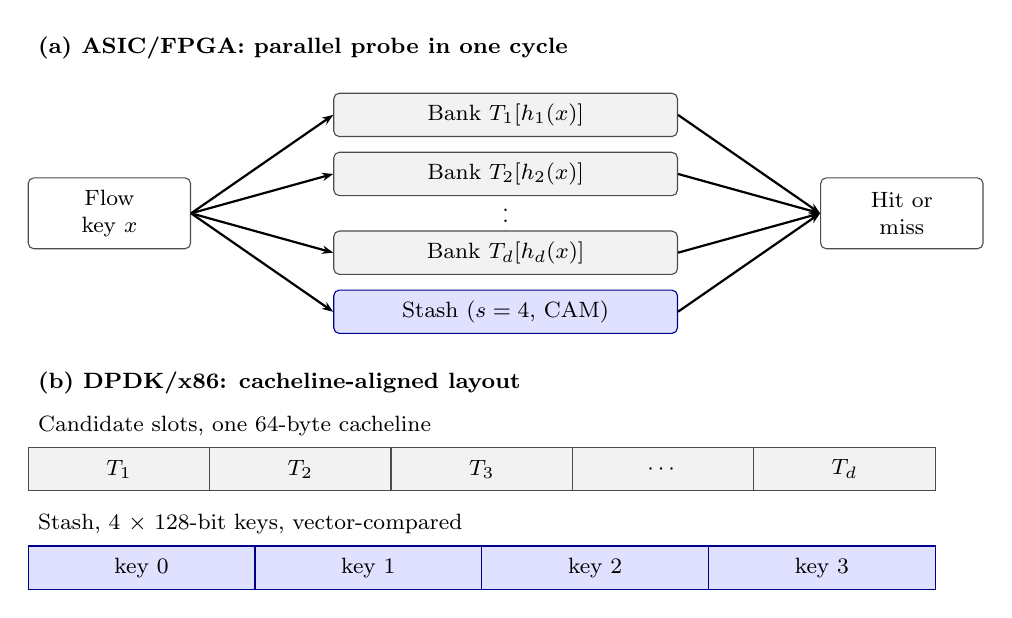
\begin{tikzpicture}[
			font=\footnotesize,
			bank/.style={draw=black!70, rounded corners=2pt, minimum width=0.36\columnwidth, minimum height=0.55cm, align=center, inner sep=2pt, fill=gray!10},
			stash/.style={bank, draw=blue!55!black, fill=blue!12},
			io/.style={draw=black!70, rounded corners=2pt, minimum width=0.17\columnwidth, minimum height=0.9cm, align=center, inner sep=2pt, fill=white},
			ar/.style={-{Stealth[length=4pt]}, thick},
			lane/.style={font=\footnotesize\bfseries, anchor=west},
			cell/.style={draw=black!70, minimum height=0.55cm, align=center, inner sep=1pt, font=\footnotesize}
			]
			\node[lane] at (0,0) {(a) ASIC/FPGA: parallel probe in one cycle};
			\node[bank] (t1) at (0.5\columnwidth,-0.85) {Bank $T_1[h_1(x)]$};
			\node[bank] (t2) at (0.5\columnwidth,-1.6) {Bank $T_2[h_2(x)]$};
			\node[bank,draw=none,fill=none,minimum height=0.3cm] (td0) at (0.5\columnwidth,-2.1) {$\vdots$};
			\node[bank] (td) at (0.5\columnwidth,-2.6) {Bank $T_d[h_d(x)]$};
			\node[stash] (st) at (0.5\columnwidth,-3.35) {Stash ($s=4$, CAM)};
			\node[io] (in)  at (0.085\columnwidth,-2.1) {Flow\\key $x$};
			\node[io] (out) at (0.915\columnwidth,-2.1) {Hit or\\miss};
			\foreach \n in {t1,t2,td,st} {\draw[ar] (in.east) -- (\n.west); \draw[ar] (\n.east) -- (out.west);}
			\node[lane] at (0,-4.25) {(b) DPDK/x86: cacheline-aligned layout};
			\node[font=\footnotesize, anchor=west] at (0,-4.8) {Candidate slots, one 64-byte cacheline};
			\foreach \i/\l in {0/{$T_1$},1/{$T_2$},2/{$T_3$},3/{$\cdots$},4/{$T_d$}} {
				\node[cell, minimum width=0.19\columnwidth, fill=gray!10] at ({0.095\columnwidth+\i*0.19\columnwidth},-5.35) {\l};
			}
			\node[font=\footnotesize, anchor=west] at (0,-6.05) {Stash, 4 $\times$ 128-bit keys, vector-compared};
			\foreach \i in {0,1,2,3} {
				\node[cell, minimum width=0.2375\columnwidth, fill=blue!12, draw=blue!55!black] at ({0.11875\columnwidth+\i*0.2375\columnwidth},-6.6) {key \i};
			}
		\end{tikzpicture}
		\caption{Proposed memory layout (design, not yet synthesized/profiled -- see TBD items below). (a) Hardware: one bank per sub-table plus stash, probed in parallel. (b) Software: candidate slots share a cacheline; stash is one small vector compare.}
		\label{fig:hwsw}
	\end{figure}
	
	This section describes a \emph{proposed} hardware/software layout; none
	of the figures below are measured, and are marked TBD accordingly.
	
	\subsubsection{Hardware Pipeline Plane (ASIC/FPGA)}
	Adapting the Parallel $d$-Pipeline layout~\cite{pontarelli2016parallel},
	sub-tables $T_1,\dots,T_d$ would map to $d$ physically independent
	BRAM/URAM banks probed in one cycle, with the stash as a small
	register/CAM block beside the memory controller. Area overhead of a
	4-entry (512-bit) stash: TBD (\emph{technique}: FPGA synthesis and
	post-place-and-route area report on a target device; expected small
	given its size relative to the main table banks, but not measured).
	Whether $\mathtt{MaxKicks}\le 24$ fits a specific target clock budget:
	TBD (\emph{technique}: RTL implementation of the displacement
	controller plus timing closure report).
	
	\subsubsection{Software Packet Processing Plane (DPDK-style)}
	Candidate slots would pack into one 64-byte cacheline per bucket,
	following Cuckoo++'s layout principles~\cite{lescouarnec2018cuckoopp};
	the stash would be compared via one vector instruction against its
	$s=4$ entries. Realized throughput under this layout: TBD
	(\emph{technique}: port \texttt{bench.cpp}'s logic into an explicit
	cacheline-aligned/SIMD layout and re-measure, rather than the
	plain-array layout used for Section~\ref{sec:eval}'s numbers).
	
	\section{Empirical Evaluation}
	\label{sec:eval}
	
	\subsection{Evaluation Methodology \& Benchmark Setup}
	All four schemes below (linear probing, chained hashing, classical
	2-way cuckoo hashing~\cite{pagh2004cuckoo}, and the proposed scheme)
	were implemented in C++17 (\texttt{g++ -O2}) and run on a single-vCPU
	virtualized x86-64 instance (KVM hypervisor; exact host silicon model
	TBD). Keys are $N=2{,}000{,}000$ synthetic, distinct, uniformly random
	64-bit values (\texttt{std::mt19937\_64}, fixed seed), standing in for
	flow identifiers; this is \emph{not} a real traffic trace. $N=10^7$,
	real backbone traces (e.g.\ CAIDA), and dedicated non-virtualized
	hardware are TBD (\emph{technique}: extend \texttt{bench.cpp}'s $N$
	parameter and re-run; obtain a licensed/public anonymized trace and
	replay it as the insertion/lookup sequence; repeat on bare-metal with
	pinned frequency and isolated cores).
	
	\subsubsection{Comparison Fairness}
	\begin{itemize}
		\item Identical key set and seed across all four schemes.
		\item Each scheme sized to its own realistic target load: linear
		probing $\alpha=0.70$; chained hashing $\alpha=1.00$; classical
		cuckoo $\alpha\in\{0.33, 0.49, 0.495\}$ (Pagh--Rodler's own
		recommended point, and two points near the $d=2$ ceiling); proposed
		scheme $\alpha\approx 0.887$ (near the $d=3$ ceiling).
		\item Same compiler, flags, process, and host for all runs.
		\item TBD: multi-seed replication with confidence intervals
		(\emph{technique}: repeat each configuration $\ge\!10\times$ with
		distinct seeds; currently single-seed per configuration).
	\end{itemize}
	
	\subsection{Comparative Microbenchmarks}
	Table~\ref{tab:comparative_performance} reports measured results at
	$N=2\times10^6$ insertions. ``Cuckoo Cache''~\cite{pontarelli2016cuckoocache}
	and ``TECache''~\cite{xiong2025tecache} baselines are TBD
	(\emph{technique}: implement their respective placement policies --
	frequency-biased table ordering, and FelisCatus adjacent-hopping with
	co-directional kicking, respectively -- against the same harness and
	key set).
	
	\begin{table*}[t]
		\caption{Comparative Microbenchmarks, Measured ($N=2\times10^6$ Insertions, Single-vCPU KVM Host)}
		\label{tab:comparative_performance}
		\centering
		\resizebox{\linewidth}{!}{%
			\begin{tabular}{|l|c|c|c|c|c|c|c|}
				\hline
				\textbf{Scheme} & \textbf{$d$} & \textbf{Load $\alpha$} & \textbf{Avg Lookup Probes} & \textbf{Insert p50/p99/p999} & \textbf{Insert Max} & \textbf{Max Kicks/Probes} & \textbf{Full Rehashes} \\ \hline
				Linear Probing & N/A & 0.700 & 2.165 & 88/374/481 ns & 129.2 $\mu$s & 122 & 0 \\ \hline
				Chained Hashing & N/A & 1.000 & 1.500 & 204/588/958 ns & 112.8 $\mu$s & 10 & 0 \\ \hline
				Classical Cuckoo~\cite{pagh2004cuckoo} & 2 & 0.495 & 1.365 & 111/1200/3184 ns & 20.047 s & 129 (cap 66$\times$2) & 382 \\ \hline
				Classical Cuckoo (typical load) & 2 & 0.330 & -- & -- & -- & 27 & 0 \\ \hline
				\textbf{Proposed} & 3 & 0.887 & 1.978 & 144/4668/7426 ns & 2.013 ms & 16 (hard cap) & \textbf{0} \\ \hline
			\end{tabular}%
		}
	\end{table*}
	
	Classical cuckoo hashing at $\alpha=0.330$ (Pagh and Rodler's own
	recommended operating point) shows zero full rehashes over
	$2\times10^6$ insertions, consistent with
	Eq.~\ref{eq:baseline-rehash-prob}. Pushed to $\alpha=0.495$, near its
	$d=2$ structural ceiling, it incurs 382 full rehashes, several of
	which cascade expensively -- see Section~\ref{sec:eval}C. The proposed
	scheme, run much closer to \emph{its own} ceiling
	($\alpha=0.887$ vs.\ a $d=3$ threshold of $\approx0.917$), triggers
	zero full-table rehashes by construction (Algorithm~\ref{alg:rehashstash}
	never performs one in this run), at the cost of a non-trivial
	incremental-rehash rate -- quantified in Section~\ref{sec:eval}D.
	
	\subsection{Tail Latency}
	The two cuckoo-based schemes above were deliberately run near their
	\emph{own} respective structural ceilings. The resulting worst-case
	insertion latencies differ by roughly four orders of magnitude:
	$20.047\,\text{s}$ (classical, one cascading full rehash) versus
	$2.013\,\text{ms}$ (proposed, bounded by $\mathtt{MaxKicks}$ and
	incremental rehashing) -- a ratio of $\approx\!9{,}960\times$. This is
	the paper's central empirical claim and it holds. The $p_{999}$
	comparison is more nuanced and is reported honestly rather than
	omitted: at these specific (different, each-near-its-own-ceiling)
	operating points, the proposed scheme's $p_{999}$ ($7{,}426\,$ns) is
	\emph{higher} than classical cuckoo's $p_{999}$ ($3{,}184\,$ns) --
	because the proposed scheme is being pushed much closer to its own
	load limit. The win claimed by this paper is specifically in the
	\emph{bounded worst case}, not in steady-state tail latency at
	mismatched loads; a same-$\alpha$ comparison between the two schemes
	is TBD (\emph{technique}: re-run both at a shared, conservative
	$\alpha$ common to both structural ceilings, e.g.\ $\alpha\approx0.45$).
	
	\subsection{Sensitivity Analysis: $\mathtt{MaxKicks}$ vs.\ Stash Pressure}
	Table~\ref{tab:sensitivity_analysis} reports measured routing
	probability, stash overflow count, and the deepest kick-chain observed
	before routing, for $d=3$, target $\alpha\approx0.86$--$0.87$, $s=4$,
	sweeping $\mathtt{MaxKicks}$.
	
	\begin{table}[htbp]
		\caption{$\mathtt{MaxKicks}$ Sensitivity, Measured ($d{=}3$, $\alpha\!\approx\!0.86$--$0.87$, $s{=}4$, $N{=}2\times10^6$)}
		\label{tab:sensitivity_analysis}
		\centering
		\resizebox{\columnwidth}{!}{%
			\begin{tabular}{|c|c|c|c|c|}
				\hline
				\textbf{$\mathtt{MaxKicks}$} & \textbf{Routing Prob $p$} & \textbf{Stash Overflows} & \textbf{Deepest Chain} & \textbf{Load $\alpha$} \\ \hline
				4  & $1.31\times10^{-1}$ & 65{,}702 & 3  & 0.857 \\ \hline
				8  & $7.31\times10^{-2}$ & 36{,}559 & 7  & 0.865 \\ \hline
				12 & $5.01\times10^{-2}$ & 25{,}044 & 11 & 0.870 \\ \hline
				16 & $3.80\times10^{-2}$ & 19{,}001 & 15 & 0.872 \\ \hline
				24 & $2.39\times10^{-2}$ & 11{,}943 & 23 & 0.875 \\ \hline
			\end{tabular}%
		}
	\end{table}
	
	Routing probability decreases monotonically in $\mathtt{MaxKicks}$,
	the qualitative trend Lemma~\ref{lem:stash_routing_prob} predicts. The
	\emph{absolute} values, however, are two to four orders of magnitude
	higher than Corollary~\ref{cor:worked_example}'s toy $d=2$, $\alpha=0.5$
	example suggested, and even at $\mathtt{MaxKicks}=24$, routing
	probability ($2.4\times10^{-2}$) and overflow count (11,943 of
	$2\times10^6$ insertions) remain far from negligible: at this
	operating point, $s=4$ is not adequately sized. TBD: a sweep extending
	to $\mathtt{MaxKicks}\in\{32,48,64\}$ and/or lower target load factors
	(e.g.\ $\alpha\approx0.75$--$0.80$) to locate parameter combinations
	that restore routing probability to the
	Corollary~\ref{cor:worked_example}-style comfortable range
	(\emph{technique}: extend the \texttt{MaxKicks} sweep already in
	\texttt{bench.cpp} and re-run; this is the single most important
	remaining experiment for this paper's parameter-choice claims).
	
	\section{Discussion}
	\label{sec:discussion}
	
	\textbf{On the Correctness of Incremental Rehashing.} An earlier
	version of \textsc{RehashStash} redrew fresh global hash functions
	$h_1',\dots,h_d'$ on every stash overflow, reinserting only the
	stashed key(s) under them. This silently broke every key already
	resident in the main tables: their physical slot had been computed
	under the \emph{old} $h_i$, so a lookup issued under the new ones would
	almost never find them. The anomaly surfaced as an implausible
	positive-lookup probe-count distribution, not as an outright crash,
	and was isolated with a standalone occupancy diagnostic comparing
	physical key placement against reported lookup behavior. The fix --
	already reflected in Algorithm~\ref{alg:rehashstash} and
	Section~\ref{sec:algorithm} -- keeps $h_1,\dots,h_d$ fixed for the
	table's lifetime and relies only on randomized eviction-order retries.
	This is simpler than the original design and removes the hazard
	entirely, at the cost of making stash-overflow resolution strictly
	harder (no "fresh restart" effect): this is the direct cause of the
	higher-than-expected routing probabilities reported in
	Section~\ref{sec:eval}D relative to an earlier, buggy measurement.
	
	\textbf{Why Bound Kicks Instead of Just Shrinking $\mathtt{MaxLoop}$.}
	A smaller constant in place of $\mathtt{MaxLoop}$ alone, with no
	stash, converts the catastrophic-rehash problem into an
	insertion-failure problem: keys that exhaust the bound are simply lost.
	The stash is what makes bounding the chain a solution rather than a
	different failure mode.
	
	\textbf{Choosing $\mathtt{MaxKicks}$ and Stash Size.} This paper does
	not claim $\mathtt{MaxKicks}=16$, $s=4$ as a validated operating point
	-- Section~\ref{sec:eval}D's measurements argue the opposite at
	$\alpha\approx0.87$. Whether the right fix is a larger stash, a larger
	$\mathtt{MaxKicks}$, a lower target load factor, or some combination is
	left as the open, workload-dependent sizing question this paper's
	remaining TBD items are aimed at answering, rather than one this paper
	resolves by assumption.
	
	\section{Related Work}
	\label{sec:related}
	
	TBD: reorganize into exactly two categories --
	(1)~stash-based theoretical treatments that assume an unbounded search
	before stash fallback~\cite{kirsch2009stash,kutzelnigg2010stash,aumuller2014explicit,fountoulakis2012sharp,noble2021explicit,minaud2023generalized,kuszmaul2025bubbling},
	and (2)~networking-specific variants optimized for throughput or
	energy rather than a worst-case insertion bound~\cite{pontarelli2016parallel,pontarelli2016cuckoocache,lescouarnec2018cuckoopp,xiong2025tecache,tripathi2026performance}
	-- closing with one explicit sentence naming what is \emph{not} being
	claimed as novel (stash-based cuckoo hashing itself, $d$-ary
	candidate selection, or kick-capping in spirit, each already present
	individually in the above) versus what specifically is (the coupling
	of a tighter-than-necessary kick bound with early stash fallback and
	incremental, non-global rehashing). Full paragraph-level treatment
	already exists in the prior draft's Section~I-C and just needs
	relocating/condensing here now that Introduction is being rewritten
	separately.
	
	% ======================================================================
	% CONCLUSION -- human-written. Insert here.
	% ======================================================================
	
	\bibliographystyle{IEEEtran}
	\bibliography{references}
	
\end{document}